%%%%%%%%%%%%%%%%%%%%%%%%%%%%%%%%%%%%%%%%%%%%%%%%%%%%%%%%%%%%%%%%%%%%%%%%%%%%%%%%%%%%%%%%%%%%%%%%%%%%%%%
%%%%%%%%%%%%%% Template de Artigo Adaptado para Trabalho de Diplomação do ICEI %%%%%%%%%%%%%%%%%%%%%%%%
%% codificação UTF-8 - Abntex - Latex -  							     %%
%% Autor:    Fábio Leandro Rodrigues Cordeiro  (fabioleandro@pucminas.br)                            %% 
%% Co-autores: Prof. João Paulo Domingos Silva, Harison da Silva e Anderson Carvalho		     %%
%% Revisores normas NBR (Padrão PUC Minas): Helenice Rego Cunha e Prof. Theldo Cruz                  %%
%% Versão: 1.1     18 de dezembro 2015                                                               %%
%%%%%%%%%%%%%%%%%%%%%%%%%%%%%%%%%%%%%%%%%%%%%%%%%%%%%%%%%%%%%%%%%%%%%%%%%%%%%%%%%%%%%%%%%%%%%%%%%%%%%%%
\section{\esp Introdução}

A indústria de ingressos já pode ser considerada digital nos dias de hoje. Não é raro que se observem eventos de entrada controlada integralmente por meio de ingressos nas telas dos \textit{smartphones}. Esta desmaterialização representa uma evolução frente ao modelo antigo -- de papel -- no qual os passes poderiam ser perdidos, roubados ou destruídos acidentalmente, demonstrando certa fragilidade de um produto que muitas vezes tem relevante valor monetário. Apesar de já ser uma indústria digitalizada, ainda se trata de um mercado centralizado.

% Apesar de já ser uma indústria digitalizada, ainda se trata de um mercado centralizado. Isto significa que um ingresso adquirido não é propriedade do comprador, mas sim representação computacional (muitas vezes em \textit{QR Code}) de registro armazenado em servidores da empresa que o distribuiu. O consumidor pode apenas apresentá-lo na entrada do evento.

Em grandes eventos, com alta demanda e forte apelo do público, existe o incentivo para que acumuladores adquiram antecipadamente um montante de ingressos com o objetivo de serem, posteriormente, vendidos por uma quantia razoavelmente maior do que os praticados oficialmente, gerando frustração tanto para os organizadores quanto para os consumidores, fãs e artistas. Esta prática de negociação dos ingressos em que os organizadores do evento não são a parte vendedora caracteriza um mercado secundário, podendo ou não ser controlado -- como no caso dos acumuladores -- pelos emissores dos ingressos \cite{singer2019golden}.

Há poucas formas de controlar este mercado secundário. Os ingressos são negociados livremente e consumidores que realmente têm interesse no evento podem ser surpreendidos com falsificações -- além dos altos preços. Não há como o consumidor se proteger ou verificar a autenticidade do ingresso, já que se trata de um mercado que normalmente não prevê a negociação de ingressos fora do escopo da venda oficial. A falta de um ambiente controlado tampouco permite uma referência de preço justo na revenda. É necessária a total e irrestrita confiança do consumidor em um negociante estranho, sem qualquer validação. Este ambiente, se controlado pelos organizadores do evento, tende a atrair mais consumidores, já que traz flexibilidade para circunstâncias em que não se possa comparecer ao evento, permitindo que os ingressos possam ser repassados à outros interessados, criando incentivos para que consumidores em dúvida acabem optando pela compra já no mercado primário. Em não se tendo uma alternativa segura de revenda, o consumidor tende a aguardar até a certeza do comparecimento, tendo que se contentar em enfrentar um mercado secundário com falsificações e altos preços -- ou abrir mão do evento.

Tornar o consumidor dono do seu ingresso é uma das formas de resolver grande parte dos problemas identificados. Livre para negociar, doar e presentar, mas de forma que a autenticidade deste ingresso pudesse ser verificada indubitavelmente por eventuais contrapartes e pelos organizadores do evento na entrada. A segurança se torna fator decisivo, principalmente em casos de razoável valor financeiro.

Redes em \textit{blockchain} resolvem este problema com o uso dos \textit{NFTs}. \textit{Tokens} em redes descentralizadas trazem transparência e flexibilidade que agregam muito ao mercado de ingressos, tornando o consumidor dono de seu ativo podendo negociá-lo livremente. Uma vez que tudo está registrado em uma rede pública, a autenticidade dos \textit{tokens} pode ser conferida durante as negociações \cite{liu2021hybrid}.

\textit{NFTs} trazem ainda mais possibilidades à este contexto. É possível incluir atributos à um \textit{token} que definirão, entre infinitas possibilidades, à quais dias do evento aquele acesso dá direito, qual é a categoria (meia entrada, inteira, cortesia etc) ou até mesmo eventuais adicionais como o \textit{open bar}, \textit{open food}, visita ao camarim ou direito à transporte para casa após o evento. Sendo assim, ao negociar aquele \textit{token}, o comprador tem visibilidade de toda a informação relevante sobre a qualidade do acesso ao evento. Não é necessária nenhuma confiança prévia entre comprador e vendedor neste tipo de negociação, cujas regras de negociação já foram previamente estabelecidas pelos emissores do \textit{NFT} e executadas pelos \textit{market places}, zerando o risco de fraudes e não cumprimento do acordo financeiro feito entre as partes \cite{liu2021hybrid}.

Por intermédio de contratos inteligentes (ou {\textit{smart contracts}), os emissores do \textit{NFT} podem definir previamente sob quais regras o mercado secundário irá operar. É possível limitar quantas transações podem acontecer para cada \textit{token}, um valor mínimo e máximo para aquele tipo específico de ingresso, além de incluir os chamados \textit{royalties} -- um percentual do valor pago pelo \textit{NFT} revertido aos criadores para cada transação feita. Estes, inclusive, acabam gerando um incentivo econômico para que não hajam transações desenfreadas envolvendo os \textit{tokens} já que reduzem a margem a cada nova negociação.

Segundo dados da consultoria alemã \citeonline{statista}, o Brasil é o segundo país com mais usuários donos de NFTs, sendo \textbf{cerca de 5 milhões de brasileiros donos de, ao menos, um \textit{NFT}}. Mesmo ficando atrás apenas da Tailândia neste mercado, podemos assumir que proporcionalmente ainda não somos usuários costumazes do mercado de \textit{NFTs} e ativos digitais. Sendo assim, é necessário implementar uma solução que embarque tanto a flexibilidade e descentralização que as \textit{blockchains} oferecem quanto a praticidade e simplicidade do uso ordinário para usuários que não tem interesse em mercados secundários ou operar \textit{NFTs} com \textit{wallets} -- apenas querem acesso ao evento.

% Uma plataforma descentralizada, imune a fraudes ou intervenções indevidas por meio de {\itshape smart contracts} na \textit{blockchain} é a base ideal para a criação de soluções que aliem segurança à liberdade. Seguindo estes critérios, a rede \textit{Ethereum} consegue atender às necessidades e contemplar as expectativas do usuário, sendo a melhor alternativa para a mediação dessas trocas \cite{liu2021hybrid}.

Este artigo pretende apresentar uma solução "híbrida" que habilite que consumidores sejam proprietários de seus ingressos, caso queiram, por meio de \textit{NFTs} na rede \textit{Ethereum}, permitindo que negociem em \textit{market places} sob regras previamente estabelecidas ou que os transfiram diretamente à quem desejarem usando suas \textit{wallets}. Para os consumidores com demandas mais simples, é proposto que se mantenha a experiência regular do mercado sem necessidade de interação direta com \textit{NFTs} -- apenas permitindo que o evento seja acessado com o \textit{QR Code} na tela do \textit{smartphone} (ou impresso). Ambos os cenários precisam ser previstos e validados na entrada do evento de forma que nenhum consumidor tenha sua experiência prejudicada em virtude do modelo de \textit{ticket} escolhido, tendo ele comprado no mercado primário ou secundário.

\section{\esp Referencial teórico}
Este artigo aborda diversos elementos da \textit{blockchain} e mais profundamente da rede \textit{Ethereum}. Para melhor compreensão, é imprescindível que determinados aspectos sejam conceituados.

\subsection{\esp \textit{Blockchain}} \label{blockchain}
\textit{Blockchain} pode ser definido como uma cadeia de blocos interligados entre si, como um livro de registros, distribuído e aberto. Inicialmente focado em moedas digitais, hoje em dia utilizado em outras aplicações além de criptomoedas e pagamentos. Existem três diferentes tipos de blockchain, que se diferenciam entre si com base em seu uso: público, privado e de consórcio \cite{bhutta2021survey}. Neste artigo focaremos em \textit{blockchains} públicas.

Quando fala-se de \textit{blockchains}, as seguintes características chaves devem ser consideradas \cite{bhutta2021survey}:

\begin{enumerate}
    \item \textbf{Descentralização:} Possivelmente o aspecto mais importante de uma \textit{blockchain}. A cadeia de blocos existe em vários computadores (\textit{nodes}) espalhados pelo mundo. Cada um destes participantes da rede ora atua como cliente, ora como servidor -- enviando ou recebendo e validando transações. A tecnologia se aproveita disso para transmitir e verificar dados sem a necessidade de uma autoridade central. O poder se concentra nos indivíduos participantes da rede, a tornando justa e consideravelmente mais segura. A confiança entre \textit{nodes} é estabelecida uma vez que há um protocolo de consenso, garantindo que uma transação é validada pela rede apenas se participantes suficientes concordarem sobre sua autenticidade. As diversas cópias da \textit{blockchain} espalhadas pelo mundo previnem a perda de informação, em detrimento de tecnologias mais centralizadas.
    \item \textbf{Transparência:} Qualquer um pode ver detalhes de cada bloco e o histórico de qualquer transação. Dada a descentralização das validações, feitas por \textit{nodes} ao redor do mundo, é necessário que todo o conteúdo dos blocos seja completamente acessível, garantindo que nada seja alterado, removido ou inserido enganosamente na cadeia de blocos.
    \item \textbf{Autonomia:} Não é necessário que haja necessariamente confiança entre os participantes da rede. As transações são garantidas pelo uso de protocolos de consenso e criptografia assimétrica.
    \item \textbf{Segurança:} A base está na criptografia assimétrica, onde pares de chaves públicas e privadas são usados para garantir a propriedade da transação, de forma que a chave privada -- sendo de conhecimento apenas de seu dono -- assegura a origem de uma transação, garantindo uma intenção genuína de interação com a rede.
    \item \textbf{Imutabilidade:} Uma vez que um dado é inserido em uma \textit{blockchain}, não poderá ser alterado. A estrutura de blocos conta com uma \textit{time stamp} e cada um deles tem seu conteúdo criptografado utilizando um algoritmo de \textit{hash}. Qualquer tentativa de mudança, não importa quão pequena, acarretará em um novo \textit{hash} -- que será detectada e rejeitada pela rede, a menos que haja consenso do contrário.
    \item \textbf{Rastreabilidade:} Uma vez que os blocos tem \textit{time stamps} e são encadeados de forma a ter uma sequência linear, é possível rastrear qualquer atividade feita ou comportamento de qualquer agente ao longo da cadeia de blocos.
    \item \textbf{Anonimato:} Apesar da rastreabilidade, qualquer agente na rede pode ser anônimo já que nenhuma informação pessoal é necessária para transacionar -- apenas uma endereço e sua chave privada. Não há como conectar um determinado endereço à uma pessoa sem que hajam informações de outras fontes.
    \item \textbf{Programabilidade:} A tecnologia é \textit{open source} e é possível desenvolver aplicações através de uma interface comum. Nem todos os \textit{blockchains} são programáveis. Exemplos são: Ethereum, Tron, Cardano, entre outros.
    \item \textbf{Automaticidade:} \textit{Smart contracts} podem automaticamente gerar transações, tomar decisões e armazenar dados. A rede é mantida e validada automaticamente utilizando um protocolo, sem intervenção manual.
\end{enumerate}

\subsubsection{\esp Carteiras (\textit{wallets})} \label{wallets}
Carteiras de \textit{blockchain} funcionam como nossas carteiras físicas, mas mantém controle de nossos criptoativos (Bitcoin, Ether, NFTs, entre outros). Tecnicamente, elas contém as chaves criptográficas necessárias para que possamos transacionar estes ativos. Se trata de um par de chaves, pública e privada, de forma que o usuário assina suas transações usando a chave privada e a rede pode verificá-las usando a chave pública. A chave pública pode ser derivada a partir da privada, mas o contrário é impossível \cite{di2020arcula}. As carteiras não armazenam os ativos em si, mas fornecem o direito de movimentá-los na rede pelo uso da chave privada.

Ainda segundo \citeonline{di2020arcula}, é possível que carteiras não tenham um único par de chaves. Com as \textit{Hierarchical Deterministic Wallets}, ou \textit{HD Wallets}, uma árvore de chaves pode ser gerada à partir de uma \textit{seed}. Esta hierarquia funciona de forma que nós mais altos podem derivar as chaves de nós mais baixos e assinar transações em seu nome, mas o contrário não deve ser possível de nenhuma maneira. Cada um dos nós tem seu próprio par de chaves e funciona como uma carteira independente. Estas carteiras oferecem uma solução interessante para aplicações que precisam gerenciar múltiplas carteiras sem que seja necessária a guarda de equivalentes \textit{seeds}.

\subsection{\esp \textit{Ethereum}} \label{ethereum}
\citeonline{antonopoulos2018mastering} define \textit{Ethereum} em seu livro como uma infraestrutura computacional \textit{open source}, descentralizada globalmente que executa programas chamados de \textit{smart contracts} e usa uma \textit{blockchain} para sincronizar e armazenar as mudanças de estado, juntamente com o criptoativo \textit{ether}. Em vez de apenas manter o balanço de unidades de criptomoedas e sua propriedade, \textit{Ethereum} mantém o estado de transações em uma memória de propósito geral, composta de chave-valor, manipulável através dos programas implantados na rede.

\textit{Smart contracts} são programas computacionais executados na \textit{Ethereum Virtual Machine} (EVM), imutáveis (após o \textit{deploy}) e determinísticos. A EVM roda como uma instância local em cada \textit{node Ethereum}, e como todas as instâncias partem do mesmo estado inicial e produzem o mesmo estado final, o sistema como um todo opera como um "único computador". Os \textit{smart contracts} são mais comumente escritos na linguagem \textit{Solidity} e podem modificar apenas o contexto de seu próprio estado, ler os contextos das transações recebidas, além de algumas informações sobre os blocos mais recentes. Seu escopo é bastante delimitado. \cite{antonopoulos2018mastering}.

\subsubsection{\esp \textit{Networks}} \label{networks}
\textit{Networks} são os diferentes ambientes acessíveis para desenvolvimento, teste ou produção. Uma conta \textit{Ethereum} é capaz de alternar entre os diferentes ambientes, mas a carteira terá um balanço não intercambiável entre eles. Dentre as redes publicamente acessíveis estão a \textit{Mainnet} e as \textit{Testnets}, sendo a \textit{Mainnet} o ambiente produtivo onde transações reais -- com \textit{ethers} de valor real -- acontecem. Já as \textit{Testnets} são usadas para testes em um ambiente parecido com o produtivo antes da implantação na \textit{Mainnet} \cite{ethereumorgnetworks}. Este artigo utilizará a \textit{Testnet} Goerli, a recomendada por padrão para fins de demonstração.

\subsubsection{\esp Validadores e protocolo de consenso}
O \textit{Ethereum} utiliza o protocolo de consenso chamado \textbf{\textit{proof-of-stake (PoS)}}. Nele, a criação de blocos é feita pelos validadores que guardam um balanço em \textit{ether} (ETH) para participarem do sistema. Um deles é escolhido aleatoriamente para criar um novo bloco, compartilha com a rede e recebe a recompensa (ETH). Com a rede operando de maneira honesta -- como na maior parte do tempo --, o bloco proposto entra no topo da cadeia de blocos e as validações seguem ao próximo bloco. Quando há discordância sobre qual bloco deveria estar no topo da cadeia (por erro ou tentativa de fraude), é escolhida a cadeia de blocos que tem o maior peso de \textit{stake} confirmando sua autenticidade \cite{ethereumorgconsensus}.

\textit{Gas fees} existem para prevenir \textit{spamming}. Cada transação tem uma medida de esforço computacional necessário para executá-la. Esta medida é traduzida em unidades de \textit{gas}. Elas são pagas na criptomoeda corrente da rede (ETH) e são queimadas após a transação executar com sucesso, servindo apenas para desincentivar que transações de intenções não legítimas sejam enviadas à rede com o único objetivo de sobrecarregá-la. É possível enviar, para determinada transação, uma \textit{priority fee (tip)} que será revertida ao validador, criando incentivo para que a transação tenha prioridade na validação e consequente inclusão em um bloco. Para que uma transação ocorra com sucesso na rede, portanto, é necessário que a carteira de origem possua em seu balanço \textit{ether} suficiente para o valor nominal da transação mais os valores das \textit{fees}, que também serão descontadas \cite{ethereumorggas}.

\subsubsection{\esp \textit{Nodes}}
\textit{Nodes} são computadores executando um \textit{client} e conectados com a rede \textit{Ethereum}. Usuários interagem com a rede através dos \textit{nodes}, que por sua vez utilizam uma das implementações de \textit{client} existentes, sendo o \textbf{Geth}, escrito em Go, o mais comum. Por meio da \textit{\textbf{Ethereum JSON-RPC Specification}} há a garantia de que a comunicação do usuário com a rede se dará da mesma maneira independentemente do \textit{client} utilizado ou do \textit{node} específico, já que estabelece uma interface que todos os \textit{clients} e, por consequência, os \textit{nodes}, precisam expor \cite{ethereumorgnodes}.

É possível executar um \textit{node} de forma independente e existem cenários onde isso é altamente desejável ou até um requisito. Uma outra forma de acessar a rede é por meio de serviços que oferecem uma abstração da infraestrutura de \textit{nodes} -- podendo fornecer ainda baixa latência e alta disponibilidade -- para cenários onde uma execução independente não é requisitada. Este artigo utilizará um destes serviços, especificamente o \textit{\textbf{QuickNode}}, capaz de se conectar na \textit{Testnet} Goerli, conforme descrito na \ref{networks}.

Simplificando a integração com os \textit{nodes}, bibliotecas de código nas mais diversas linguagens abstraem a \textit{\textbf{Ethereum JSON-RPC Specification}} de forma que o programador seja capaz de interagir com a rede na linguagem de programação de sua escolha \cite{ethereumorgrpc}. Será utilizado neste artigo o \textit{\textbf{Nethereum}}, para .NET.

\subsubsection{\esp \textit{Tokens}}
Por meio de \textit{smart contracts}, a \textit{Ethereum} abre possibilidades para que exista não só a criptomoeda nativa -- \textit{ether} --, mas também \textit{tokens} diversos na rede. Eles podem ser definidos, de forma genérica, como abstrações baseadas em \textit{blockchain} que podem ser possuídos e representam ativos, moeda, direitos de acesso ou voto, colecionáveis, \textit{equity}, entre outras infinitas aplicações \cite{antonopoulos2018mastering}.

Ainda segundo \citeonline{antonopoulos2018mastering}, \textit{tokens} podem ser fungíveis ou não fungíveis, sendo fungibilidade a capacidade de uma unidade de \textit{token} ser trocada por outra sem nenhuma diferença de valor ou função. Embora valha ponderar que num ambiente completamente rastreável como é a \textit{blockchain}, o histórico de um \textit{token} pode diferenciá-lo dos demais na prática, por razões imprevisíveis, mesmo sendo tecnicamente fungível. Tokens não fungíveis, por outro lado, representam, cada, um item tangível ou intangível não intercambiável e são comumente chamados de \textit{NFTs (non-fungible tokens)}.

Apesar de \textit{smart contracts} poderem ser escritos conforme desejado, \citeonline{antonopoulos2018mastering} defende que sejam utilizados os padrões estabelecidos pela comunidade e aprimorados pela \textit{\textbf{OpenZeppelin}}, uma plataforma \textit{open source} que oferece uma biblioteca de \textit{standards} com aprimoramentos de segurança e funcionalidade. \textit{Ethereum Request for Comments (ERC)} é o mecanismo pelo qual a comunidade \textit{Ethereum} estabelece padrões, sendo os \textbf{ERC20} e \textbf{ERC721} os mais aceitos para \textit{tokens} fungíveis e não fungíveis, respectivamente. Utilizar estes padrões significa se aproveitar da maturidade de um código amplamente utilizado e testado, assim como um ecossistema integrado capaz de interagir com os contratos definidos por eles. Este artigo implementatá um \textit{token} adotando o padrão \textbf{ERC721} da biblioteca \textit{\textbf{OpenZeppelin}}.

Na interface definida pela \textbf{ERC721}, o processo de geração de \textit{tokens} é chamado de \textit{\textbf{mint}}, e a destruição de \textit{tokens}, por qualquer razão conveniente, é chamada de \textit{\textbf{burn}}.

O padrão \textbf{ERC721} possibilita que cada \textit{token} gerado tenha \textbf{seu próprio Id} e armazene uma url que direciona à um arquivo de metadados no formato \textit{JSON} contendo informações adicionais sobre aquele ativo. Tais informações incluem, principalmente, um nome, descrição, imagem, url externa e atributos formados por elementos chave-valor livremente definidos pelo criador. A utilização deste arquivo agrega tangibilidade ao ativo, já que é utilizado por plataformas de exibição de NFTs, além de \textit{market places}, trazendo ao usuário a possibilidade de concretizar visualmente uma representação digital em uma \textit{blockchain}. Uma vez que o arquivo em si não está armazenado na cadeia de blocos, e portanto não está limitado por sua imutabilidade, é possível ao criador fazer alterações em seu conteúdo gerando no usuário, quando conveniente, a sensação de vivacidade, movimento, evolução de seu ativo embora ele permaneça estático na \textit{blockchain} em si.

\subsubsection{\esp \textit{Market places}} \label{marketplace}
Se trata de um espaço para negociação de \textit{tokens}, fungíveis e não fungíveis. Este artigo focará em \textit{market places} especializados em \textit{NFTs}, mais especificamente o \textbf{OpenSea} \footnote{Disponível em \url{https://opensea.io/}}, o primeiro e maior deles. É possível fazer login na plataforma conectando uma \textit{wallet}, como a \textbf{Metamask}, sem necessidade de se identificar pessoalmente, podendo permanecer ainda anônimo na rede. Os ativos em posse da \textit{wallet} são automaticamente identificados e aparecem como custódia da conta, podendo transferi-los livremente à outro endereço ou colocá-los a venda por um preço determinado sujeito à contrapropostas.

% \subsubsection{\esp \textit{Royalties}} \label{royalties}
% O \textit{ERC2981} estabelece o padrão para o pagamento de \textit{royalties}. Ao implementar a especificação, um \textit{smart contract} define um percentual da venda a ser pago ao criador em cada negociação de um \textit{token}. Isto permite ao emissor, entre outras possibilidades, diminuir o preço da venda inicial do ativo na expectativa de ganhos no mercado secundário, ou até investir na publicidade de seus \textit{NFTs} de forma a potencializar o interesse e consequente liquidez.

% Mesmo que um \textit{smart contract} implemente este padrão, o pagamento dos \textit{royalties} não é forçado pelo contrato em si, sendo sua aplicação de deliberação dos \textit{market places} -- que intermediam as negociações. Porém, a partir de novembro de 2022, o \textit{\textbf{OpenSea}} criou sua própria especificação, que foi chamada de \textit{"fees on-chain"}. Este padrão, juntamente ao \textit{ERC2981}, cria um mecanismo onde o \textit{token} só pode ser negociado por \textit{market places} que deliberem à favor do pagamento das taxas de criador, de forma que o próprio \textit{OpenSea} não mais executará os pagamentos em \textit{tokens} que não implementem o padrão supracitado -- evitando que haja uma preferência dos usuários por negociar em outros ambientes que não executem os \textit{royalties}, tornando a negociação nestes desinteressante para criadores que desejem receber as taxas \cite{opensearoyalties}.

% \subsection{\esp \textit{QR Code}}
% \textit{Quick Response Code}, ou \textit{QR Code}, se trata de uma matriz bidimensional codificada composta por módulos comumente pretos arranjados em um quadrado de fundo branco. Criado em 1994, foi desenhado para ser lido muito rapidamente e especialmente por smartphones, o motivo do grande crescimento de sua adoção ao redor do mundo \cite{tiwari2016introduction}.

% \subsection{\esp \textit{JWT}}
% O padrão definido pela \textbf{RFC 7519}, mais conhecido como \textit{JSON Web Token (JWT)}, estabelece uma técnica de transmitir objetos \textit{JSON} entre partes de forma segura, compacta e auto-contida, o tornando especialmente adequado para ambientes restritos como o \textit{HTTP}. Para casos onde apenas a integridade é necessária, os dados podem ser simplesmente assinados com a utilização do algoritmo HMAC. Caso, além da integridade, seja requisitado também que os dados não sejam visíveis aos usuários, devem ser criptografados utilizando criptografia assimétrica \cite{jones2015json}. Seu uso mais difundido é para autorização de aplicações, que será a utilização deste artigo, já que é útil para armazenar permissões de acesso de forma que o servidor pode confiar no \textit{JWT} enviado pelo \textit{client} sem que seja necessária uma outra fonte de permissões do usuário a cada requisição -- uma vez que o \textit{token} é assinado, garantindo sua autoria e incorruptibilidade.

% \subsection{\esp Bancos de dados relacionais}
% Conforme defendido por \citeonline{jatana2012survey}, o modelo relacional é benéfico quando se tem os requisitos de confiabilidade, flexibilidade, robustez e estalabilidade. Apesar de não ser o mais adequado para altíssimos e imprevisíveis volumes de dados, se mostra atrativo para cenários mais estruturados. Permite que partes de dados sejam deliberadamente organizados em tabelas próprias de forma que a base de dados possa ser visualizada dinamicamente e sob demanda, podendo variar a relação entre as tabelas conforme necessidade de consulta. Por ser o modelo que melhor serve aos requisitos deste artigo utilizou-se o modelo relacional, pelo uso específico do \textit{\textbf{SQL Server}}.

\section{\esp Trabalhos relacionados}

As possibilidades inerentes a execução de \textit{smart contracts} são discutidas há alguns anos. Essa evolução é debatida formalmente desde o primeiro estudo sobre a criação de redes descentralizadas de dados por \citeonline{haber1990time}, que tentaram prever como seria a criação de uma “\textit{digital safety-deposit box}”, responsável por armazenar dados e torná-los incorruptíveis. Essa definição primitiva de uma \textit{blockchain} se preocupou em assegurar que documentos corporativos, assim como quaisquer alterações, fossem mantidos através dos tempos, permitindo não só a manutenção da gestão de conhecimento de uma organização, mas domínio completo da segurança desses dados. 
Já era de se esperar que essa nova modalidade não se resumisse a documento, já que qualquer cadeia de \textit{bits} pode se tornar algo único e inviolável. É por essa possibilidade que, apesar de imprevisíveis e recheados de críticas, o surgimento de \textit{NFTs} não é novidade para quem acompanha o desenvolvimento desse criptosistema desde o início.

É em meio a essa inovação que a rede \textit{Ethereum}, uma plataforma que aplica a tecnologia blockchain para execução de contratos de naturezas diversas, consegue se manter em destaque ao cumprir os principais requisitos de um intermediário de acordos digitais, permitindo que pessoas e empresas em contexto global codifiquem e apliquem acordos complexos sem confiança \cite{tikhomirov2018smartcheck}. Os \textit{smart contracts}, transações codificadas que só ocorrem a partir do cumprimento das solicitações das partes envolvidas, tornam a confiança fator quase desprezível nas interações financeiras.

Essa dinâmica foi descrita por \citeonline{tikhomirov2018smartcheck} com objetivo investigar como a tecnologia \textit{blockchain} tem sido envolvida no mercado de bilheterias \textit{online} para resolver as recorrentes fraudes que acometiam os consumidores e como a rede \textit{Ethereum} se mantém em destaque como fundamento dessa solução de mercado. O autor expõe que, através da descentralização e da transparência, características-chave dessa plataforma, a predominância de cambistas pode ser amenizada. O dispositivo desenhado para o projeto é chamado de \textit{Smart Check} e tem como função principal verificar a validação dos contratos estabalecidos por meio de uma série de testes não providos pela plataforma automaticamente.

Em uma perspectiva mais comercial, \citeonline{singer2019golden} entrevista diversos produtores musicais e confirma sua hipótese de que o mercado de bilheterias está monopolizado e, portanto, distorcido por empresas que se favorecem com a presença de cambistas e acumuladores. O autor encontrou evidências de que a maior distribuidora de ingressos dos Estados Unidos, a \textit{TicketMaster}, desenvolveu um site de vendas paralelo para a manutenção do mercado secundário, permitindo que revendedores comprassem quantidades ilimitadas de ingressos. A solução proposta também envolve a inserção da rede \textit{Ethereum} para compra e venda de ingressos, mas sem o desenvolvimento de aplicações ou dispostivos próprios que possibilitem essa intermediação.

No contexto tecnológico atual, a indústria que promove a integração da criptografia nos mais diversos nichos de mercado tem impactado o dia-a-dia de seus consumidores, mas essa fusão dificilmente é percebida ou usada diretamente por eles. Aspectos de segurança e privacidade já minimizaram seus respectivos problemas, mas é na possibilidade dos contratos e acordos pessoais descentralizados e invioláveis que as dores de mercado podem ser solucionadas, já que esse alto nível de transparência não tem precedentes segundo   \citeonline{bhutta2021survey}.

\citeonline{liu2021hybrid} apresenta uma proposta de soluções híbridas. O problema abordado também envolve o mercado secundário de ingressos e, com o acréscimo dos problemas de privacidade do consumidor, a sugestão exposta busca combinar os diferentes tipos de \textit{blockchain} (público e privado) para diferentes situações possíveis. O autor investiga as nuances desse problema através de exemplos reais de vazamento de dados do consumidor e aponta que, apesar de todos esses inconvenientes serem previstos pela indústria, a solução proposta pelos organizadores de eventos não é tão confiável quanto um sistema sustentado por uma rede \textit{blockchain} pode ser. Apesar de contemplar os principais obstáculos desse mercado, a implementação dessa solução não é descrita com muitos detalhes, já que é dito previamente que o projeto expõe uma arquitetura abstrata que deve sofrer ajustes.

A proposta de implementar \textit{tokens} não fungíveis em ingressos também foi tema de \citeonline{regner2019nfts} e \citeonline{howell2022nft}, focados em justificar e fundamentar essa ideia para o mercado. Mesmo que sem demonstrações práticas de uma aplicação ou \textit{website} próprios, os autores demonstraram como a inserção de \textit{NFTs} poderia ocorrer nessas transações e buscaram apoio de especialistas para avaliar os resultados.

\citeonline{khanblockchain}, diferentemente dos outros trabalhos, dá prioridade para a rede \textit{blockchain hyperledger}, mas também não desenvolve plataformas próprias. O autor busca fundamentar a emissão de ingressos em um criptossistema e realizar as trocas por lá, elucidando como esse movimento pode amenizar a presença do mercado ilegal e dar maior visibilidade para o consumidor, e reforça não acreditar que a criptografia é a solução final, mas apenas um dificultador de fraudes e invasões de privacidade.

É notável que a implementação da tecnologia \textit{blockchain} nos mais diversos mercados e serviços é uma tendência sem previsão de acabar. Suas possibilidades não são apenas úteis, mas, muitas vezes, essenciais para o bom funcionamento de um mercado. Este artigo busca, assim como os trabalhos citados acima, elucidar a importância dessa evolução e, principalmente, introduzir o funcionamento de uma aplicação exclusiva.

\section{\esp Proposta}

Afim de ilustrar ainda mais o problema identificado, promoveu-se uma pesquisa (apêndice \ref{pesquisa}) com intuito de investigar o comportamento dos consumidores de ingressos.

85,7\% dos entrevistados já deixaram de comprar ingressos em plataformas não oficiais por medo de sofrer golpes. Ainda assim, 42,9\% disseram já ter comprado em tais condições, o que indica uma demanda por compras no mercado secundário, inibida pelos riscos do modelo informal.

90,5\% dos participantes enxerga \textit{NFTs} como uma solução a este cenário. Conforme exibido no Gráfico 1, todos que já sofreram golpes em compras de ingressos estariam dispostos a usar \textit{tokens} digitais como uma solução a este problema. Entre os que já deixaram de comprar ingressos em meios clandestinos por medo de golpes, 89\% entendem que \textit{NFTs} podem ser uma solução para o mercado de \textit{tickets}.

\begin{center}
    \centering
    \textbf{Gráfico 1 - Probabilidade de adesão ao NFT}
    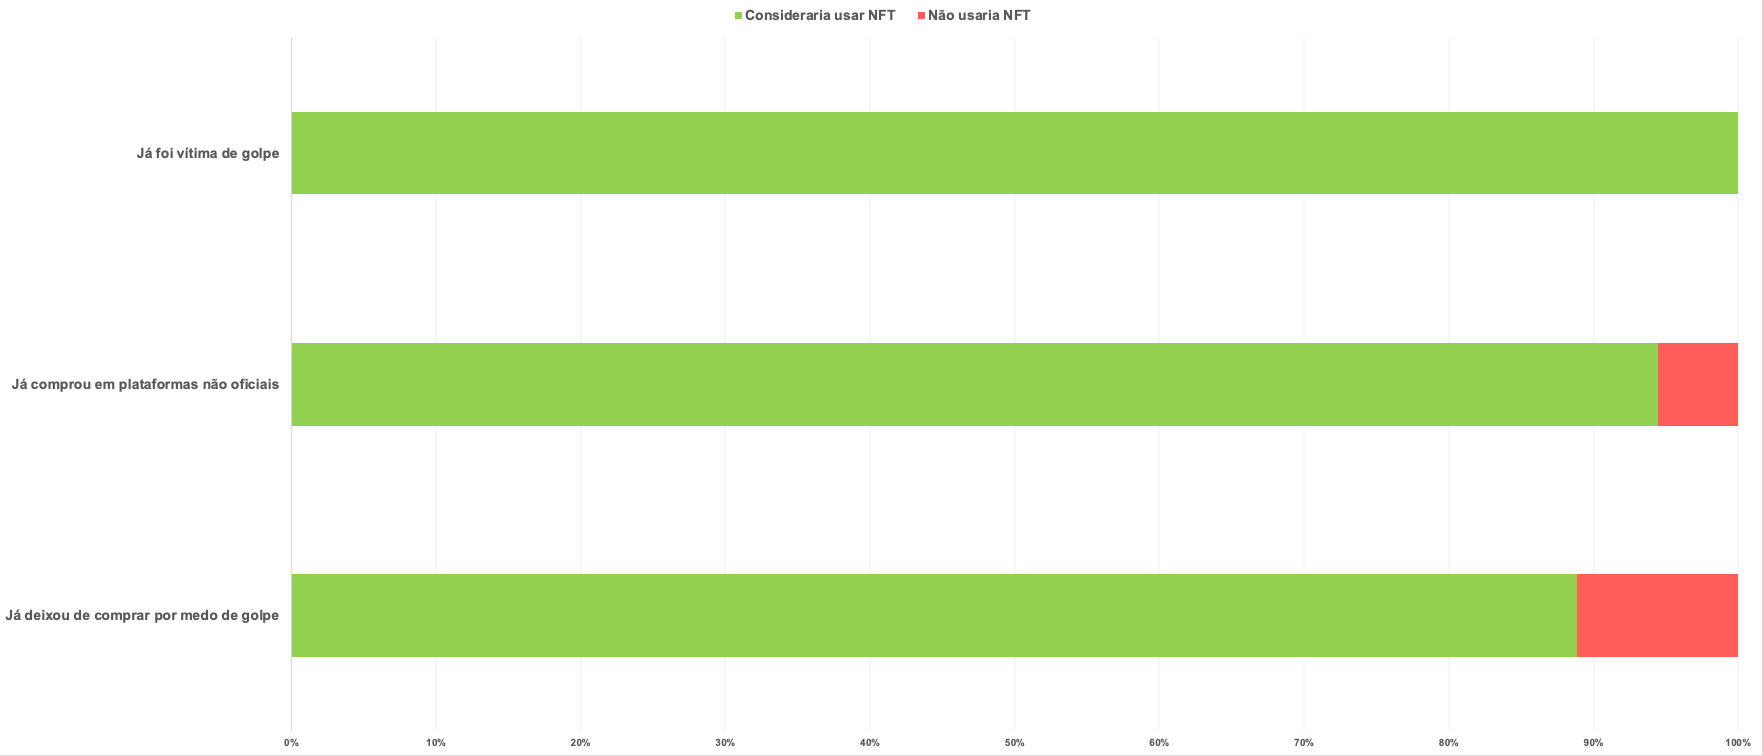
\includegraphics[scale=0.24]{figuras/grafico-pesquisa.png}
    \label{graf:grafico-pesquisa}
\end{center}

A alta aderência aos \textit{tokens}, identificada pela pesquisa, consolida um direcionamento de solução na qual a \textit{blockchain} seria protagonista, dadas as suas características. Desta forma, será descrita uma proposta de implementação prática dos conceitos estabelecidos.

% \subsection{\esp Cadastro de usuários}

Os papeis envolvidos nos fluxos da aplicação estão contempladas em 3 \textit{roles} de usuário:
\begin{enumerate} 
    \item \textit{\textbf{Customer}}: usuário consumidor que interage com a aplicação visualizando eventos e comprando ingressos; 
    
    \item \textit{\textbf{Backoffice}}: responsável pelo cadastro e gerenciamento de eventos, além do cadastro de novos usuários \textit{Backoffice} e \textit{Gatekeeper}; 
    
    \item \textit{\textbf{Gatekeeper}}: faz a validação do ingresso (representado pelo \textit{QR Code}) no momento do acesso ao evento. 
\end{enumerate}

Durante o registro, o consumidor informa o endereço de sua \textit{wallet} proprietária, para onde os \textit{tokens} serão eventualmente transferidos caso assim seja desejado.

É gerado automaticamente para cada usuário um endereço de \textit{wallet} interno, onde ficam todos os \textit{NFTs} de ingressos adquiridos. Esta carteira fica alocada ao consumidor, mas seu controle ainda é feito pela aplicação, de forma que o consumidor não tem a chave privada. Para que tome posse efetiva do \textit{token} -- caso queira --, deverá solicitar a transferência para o endereço de sua wallet proprietária informado no cadastro.
    
% \subsection{\esp Estrutura da \textit{wallet} interna}

A aplicação usa uma \textit{HD Wallet} cujo primeiro endereço da hierarquia é reservado para os deploys de \textit{smart contracts}. Os demais endereços são alocados para os consumidores, estando todos eles no mesmo nível hierárquico. A carteira interna serve ao propósito de organizar os ativos emitidos -- já que tem um espaço dedicado a cada consumidor -- assim como oferecer endereços únicos e portanto identificáveis para que o consumidor possa transferir ativos de volta à custódia interna.

% \subsection{\esp \textit{Login}}

A senha informada pelo usuário no cadastro é armazenada criptografada, utilizando uma função \textit{hash} criptográfica \textit{SHA-256}, para que o texto original da senha permaneça em segurança mesmo que os dados sejam eventualmente comprometidos. O processo de \textit{login} se dá pela comparação entre o \textit{hash} da senha informada e a senha já armazenada no banco de dados. Em caso de sucesso, o usuário receberá um \textit{JWT} que garantirá seu acesso às demais rotas do sistema. O \textit{JSON Web Token} tem duração de 2 horas e estabelece uma técnica de transmitir objetos \textit{JSON} entre partes de forma segura, compacta e auto-contida, o tornando especialmente adequado para ambientes restritos como o \textit{HTTP}, contendo, além do \textit{username}, a \textit{role} daquele usuário para que seja feita a proteção de rotas não autorizadas.

% \subsection{\esp Criação de eventos}

A criação dos eventos é feita pelo usuário \textit{Backoffice}, tendo a entidade do Evento atributos como nome, descrição, datas (início e fim), imagem, local, além dos tipos de ingressos disponíveis bem como seus preços. Os tipos de ingressos posíveis são:

\begin{enumerate} 
    \item \textit{\textbf{Regular}}: ingresso comum para o público geral; 
    
    \item \textit{\textbf{Student}}: estudante;
    
    \item \textit{\textbf{Staff}}: funcionários do evento;
    
    \item \textit{\textbf{Complimentary}}: cortesias deliberadas.
\end{enumerate}

Cada um dos tipos de ingressos contém, igualmente, seus próprios atributos, como data de início e fim do acesso, preço e oferta total de ingressos que ficarão disponíveis para venda.

\begin{figure}[ht]
    \centering
    \caption{Fluxo de criação de evento}
    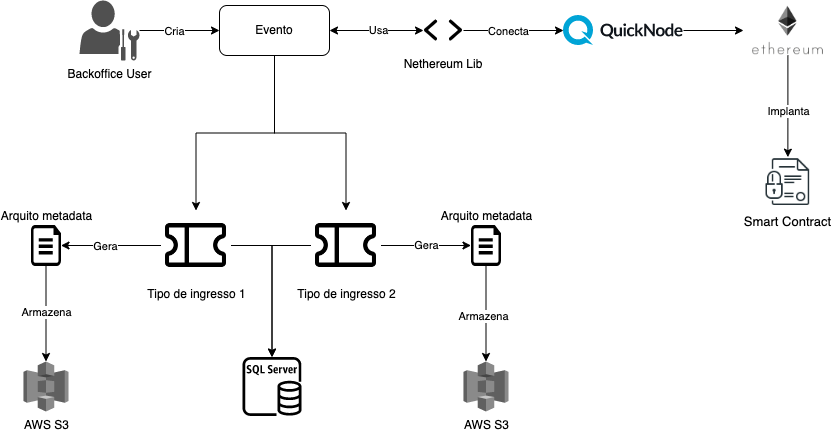
\includegraphics[scale=0.37]{figuras/event-creation.png}
    \label{fig:event-creation}
\end{figure}

% \subsubsection{\textit{Deploy} do \textit{smart contract}}

A implantação do \textit{smart contract}, conforme exibido na Figura \ref{fig:event-creation}, é feita por intermédio da biblioteca \textit{Nethereum}, se conectando com o serviço \textit{QuickNode} que fornece os \textit{nodes} de conexão à rede \textit{Ethereum}. O código do \textit{smart contract} herda funcionalidades da biblioteca de padões \textit{OpenZeppelin}. Os requisitos não demonstraram necessidade de customização, sendo suficiente criar um contrato que implementasse os seguintes elementos da biblioteca: ERC721, ERC721Enumerable, Ownable, ERC721URIStorage.

% \begin{verbatim}
%     contract TicketToken is 
%         ERC721, 
%         ERC721Enumerable, 
%         Ownable, 
%         ERC721URIStorage { }
% \end{verbatim}

Cada evento tem seu próprio \textit{smart contract} e a rede retorna, após o \textit{deploy}, o endereço do contrato na rede que será armazenado no banco de dados juntamente com os demais dados do evento e seus tipos de ingresso que geram, cada, um arquivo de metadados em JSON contendo atributos relevantes do evento e da tipagem do ingresso, além da referência de uma imagem. O arquivo serve para uso dos \textit{market places} e demais plataformas de exibição de \textit{NFTs} e é armazenado no AWS S3, um serviço que fornece \textit{storaging} de alta disponibilidade e permite gerar \textit{urls} públicas de acesso, funcionalidade ideal para o fluxo proposto.

% \subsection{\esp Visualização dos eventos disponíveis}

Os consumidores podem visualizar os eventos disponíveis e escolher quais deles comprar. Cada evento pode ter diversos tipos de ingresso, tornando sua disponibilidade uma razão das disponibilidades dos seus tipos de ingressos relacionados, que por sua vez terão sua venda limitada a data do início cadastrada.

% \subsection{\esp Compra do ingresso}

\begin{figure}[ht]
    \centering
    \caption{Fluxo de compra de ingresso}
    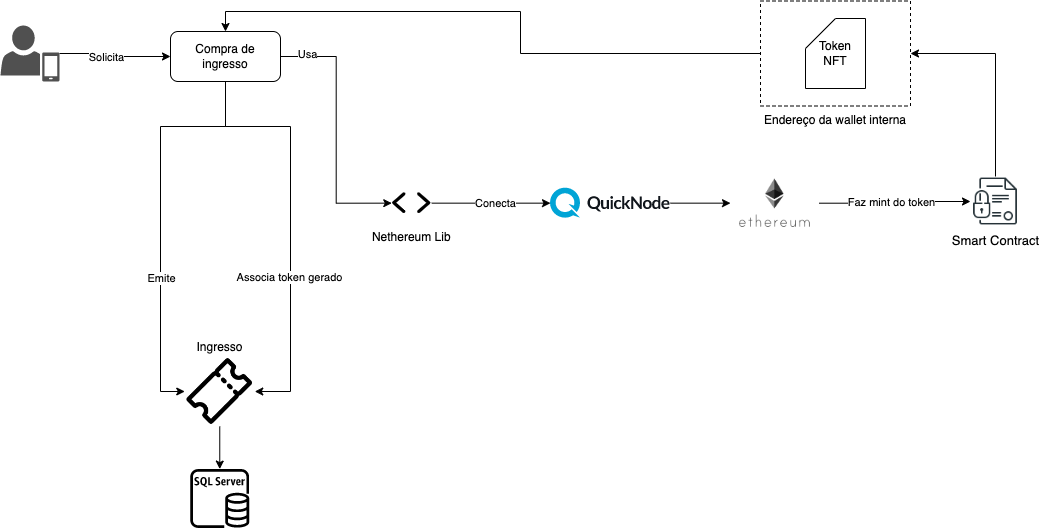
\includegraphics[scale=0.37]{figuras/ticket-buy.png}
    \label{fig:ticket-buy}
\end{figure}

Uma vez escolhido o evento e o tipo de ingresso desejado pelo consumidor, a compra será finalizada de acordo com as formas de pagamento definidas pelo organizador do evento. Este artigo não tem como objetivo propor formas de pagamento tampouco incluir uma implementação de pagamentos na aplicação. Deste passo em diante será assumido que o ingresso foi adquirido pelo consumidor mediante qualquer bem aceito pelo evento - seja ele dinheiro, cartão, cortesia ou qualquer outro.

O processo de compra envolve garantir que há disponibilidade de ingressos disponíveis que o evento assim como o tipo de ingresso escolhido, ainda tem oferta de ingressos disponíveis. Com a operação autorizada será feito o \textit{mint} do \textit{NFT} utilizando o endereço interno alocado para o consumidor. Durante o \textit{mint} também é informado ao \textit{smart contract} a \textit{url} do arquivo de metadados a ser considerado para aquele \textit{token}. Para tal, será consultado o arquivo correspondente ao tipo de ingresso gerado e consequentemente informado como parâmetro na transação. A conclusão do processo acarreta no \textit{ticket} estar acessível na conta do consumidor, assim como o \textit{token} devidamente alocado em seu endereço interno.

% Um modelo do arquivo de metadados pode ser visto à seguir:
% \begin{verbatim}
% {
%     "name": "Nome do evento 2023",
%     "description": "Descrição completa do evento",
%     "external_url": "",
%     "image": "https://url-da-imagem-token.com",
%     "attributes":
%     [
%         {
%             "trait_type": "Location",
%             "value": "Local do evento"
%         },
%         {
%             "trait_type": "Date", 
%             "value": "Datas de início e fim do evento"
%         },
%         {
%             "trait_type": "Qualification",
%             "value": "Student"
%         },
%         {
%             "trait_type": "Access",
%             "value": "Pass (All days) - Open bar"
%         }
%     ] 
% }
% \end{verbatim}

\section{\esp Resultados}
Serão demonstrados os resultados dos fluxos práticos expostos na proposta. Nesta seção, vários endereços da \textit{blockchain} serão exibidos \footnote{Enfatiza-se que não se use quaisquer desses endereços para reproduzir em ambiente próprio os cenários aqui explicitados -- ainda que se tratem de transações feitas em rede \textit{testnet} -- e que nunca se utilize dinheiro real em cenários de teste.}.

Para acompanhar as movimentações realizadas via \textit{blockchain}, será utilizado o \textit{\textbf{Ehterscan}} \footnote{Disponível em \url{https://etherscan.io/}}, que é um \textit{block explorer} capaz de rastrear, em tempo real, as transações de um \textit{token} assim como todas as operações de um endereço específico no decorrer da cadeia de blocos.

\subsection{\esp Deploy do smart contract}

A transação foi devidamente registrada na \textit{blockchain}, conforme visto na Figura \ref{fig:deploy-smartcontract}, e um endereço \footnote{Endereço: 0xd9559c5003d64af10cb65b72b419b49a02bb44ef} foi atribuído ao contrato.

\begin{figure}[ht]
    \centering
    \caption{Etherscan - \textit{Contract Creation}}
    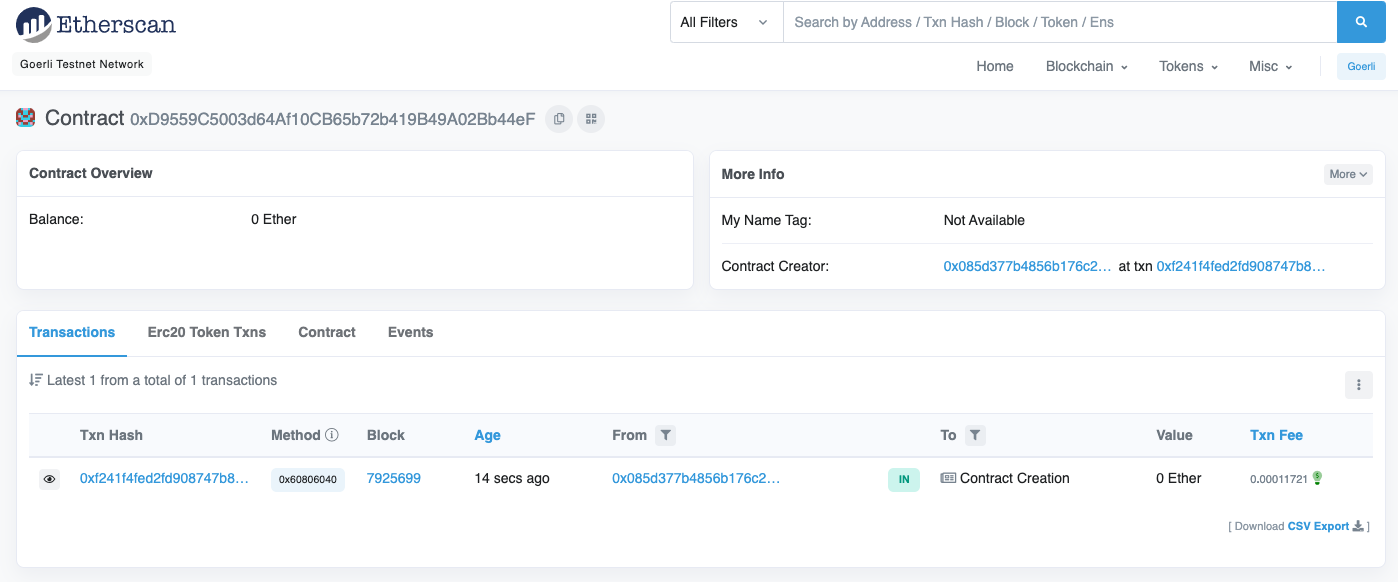
\includegraphics[scale=0.35]{figuras/deploy-smartcontract.png}
    \label{fig:deploy-smartcontract}
\end{figure}

\subsection{\esp Pós-compra e utilização do ingresso} \label{ticket-utilization}

A compra, desta forma, disparou o processo de \textit{mint}, que terminou alocando o ativo na carteira interna atribuída ao consumidor \footnote{Endereço: 0x5bfa4dc51e20317f49e44618c2d1678682c88732}, conforme evidenciado na Figura \ref{fig:mint-token}. Já é possível visualizar alguns atributos do \textit{token}, tais como o nome, o \textit{Token ID}, o endereço de destino, além de \textit{fees}. Um detalhamento de transação pode ser verificado na Figura \ref{fig:mint-token-details}.

\begin{figure}[ht]
    \centering
    \caption{Etherscan - \textit{Safe Mint method}}
    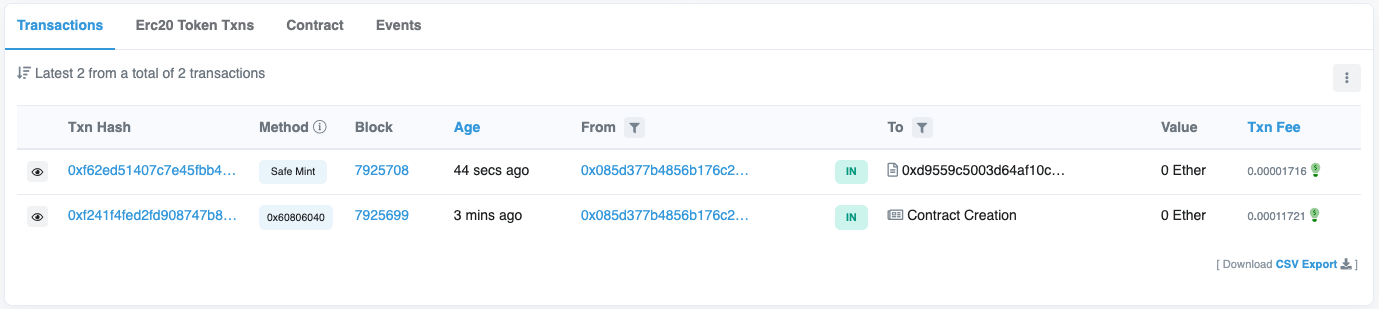
\includegraphics[scale=0.3]{figuras/mint-token.png}
    \label{fig:mint-token}
\end{figure}

\begin{figure}[ht]
    \centering
    \caption{Etherscan - \textit{Mint transaction details}}
    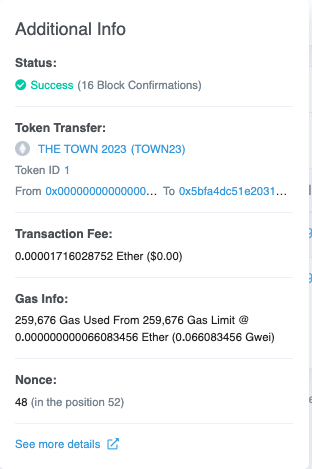
\includegraphics[scale=0.3]{figuras/mint-token-details.png}
    \label{fig:mint-token-details}
\end{figure}

Juntamente às demais informações do evento e do ingresso, o consumidor acessa um \textit{QR Code}, que será utilizado para validar o ingresso na entrada do evento, contendo o código do consumidor juntamente com o código do ingresso. Por segurança, estas informações são encriptadas com criptografia assimétrica, no uso da biblioteca RSA, nativa do .NET.

Na entrada do evento, o usuário \textit{\textbf{Gatekeeper}} faz a leitura do \textit{QR Code} e permite ou não o acesso com base na resposta da validação.

Nesta validação, é decriptado o conteúdo do \textit{QR Code} afim de extrair os códigos do consumidor e do ingresso. Primeiro é checado se aquele ingresso já foi utilizado, além de garantir que o consumidor informado é ainda dono daquele \textit{ticket}. Estas validações são feitas a nível de banco de dados. A partir daí o ingresso é sinalizado como já utilizado, e na sequência é feita a validação a nível de blockchain: confirma-se que o dono do \textit{token} correspondente àquele ingresso é realmente o consumidor informado. Isso é feito garantindo que o \textit{NFT} está no endereço interno da carteira daquele consumidor -- ou seja, temos a garantia de que não houve uma transferência para a \textit{wallet} proprietária do usuário, de onde ele poderia transferir livremente. Estas validações são executadas rapidamente, sendo retornado o resultado para o \textit{Gatekeeper} seja de falha ou sucesso.
    
\subsection{\esp Transferência do ingresso}

O consumidor pode também transferir o token contendo o ingresso para o endereço de \textit{wallet} proprietária \footnote{Endereço: 0xCa2acA0E413A6cbbC096F03E0896D28867f431b4}, além de simplesmente utilizar o ingresso na entrada do evento. Ao solicitar a transferência, é validado se o ingresso relacionado àquele ativo já foi utilizado no evento, caso no qual não poderá ser concluída a transação. Com a execução, o \textit{token} já aparecerá disponível na \textit{wallet} proprietária. O ingresso, armazenado no banco de dados, constará como "sem dono" enquanto o \textit{NFT} correspondente estiver fora dos domínios de um dos endereços da árvore gerada pela \textit{wallet} do sistema. Portanto, se qualquer consumidor tentar acessar o evento utilizando este ingresso, a validação falhará (conforme regras descritas na \ref{ticket-utilization}).

É possível visualizar a custódia do ativo por meio da plataforma \textit{\textbf{OpenSea}}, acessando com a \textit{wallet} proprietária, de forma que o \textit{token} é automaticamente identificado e exibido no perfil. O consumidor está, a partir daí, livre para transferir e negociar seu ingresso representado pelo ativo digital em sua carteira, evidenciado na Figura \ref{fig:opensea}. A partir deste momento, o \textit{QR Code} gerado anteriormente para o ingresso não mais funcionará, uma vez que a validação feita pelo \textit{Gatekeeper} leva em consideração a presença do \textit{NFT} no endereço interno do consumidor, elemento que passa a não ser mais verdadeiro.

\begin{figure}[ht]
    \centering
    \caption{\textit{OpenSea} - Detalhe do ativo}
    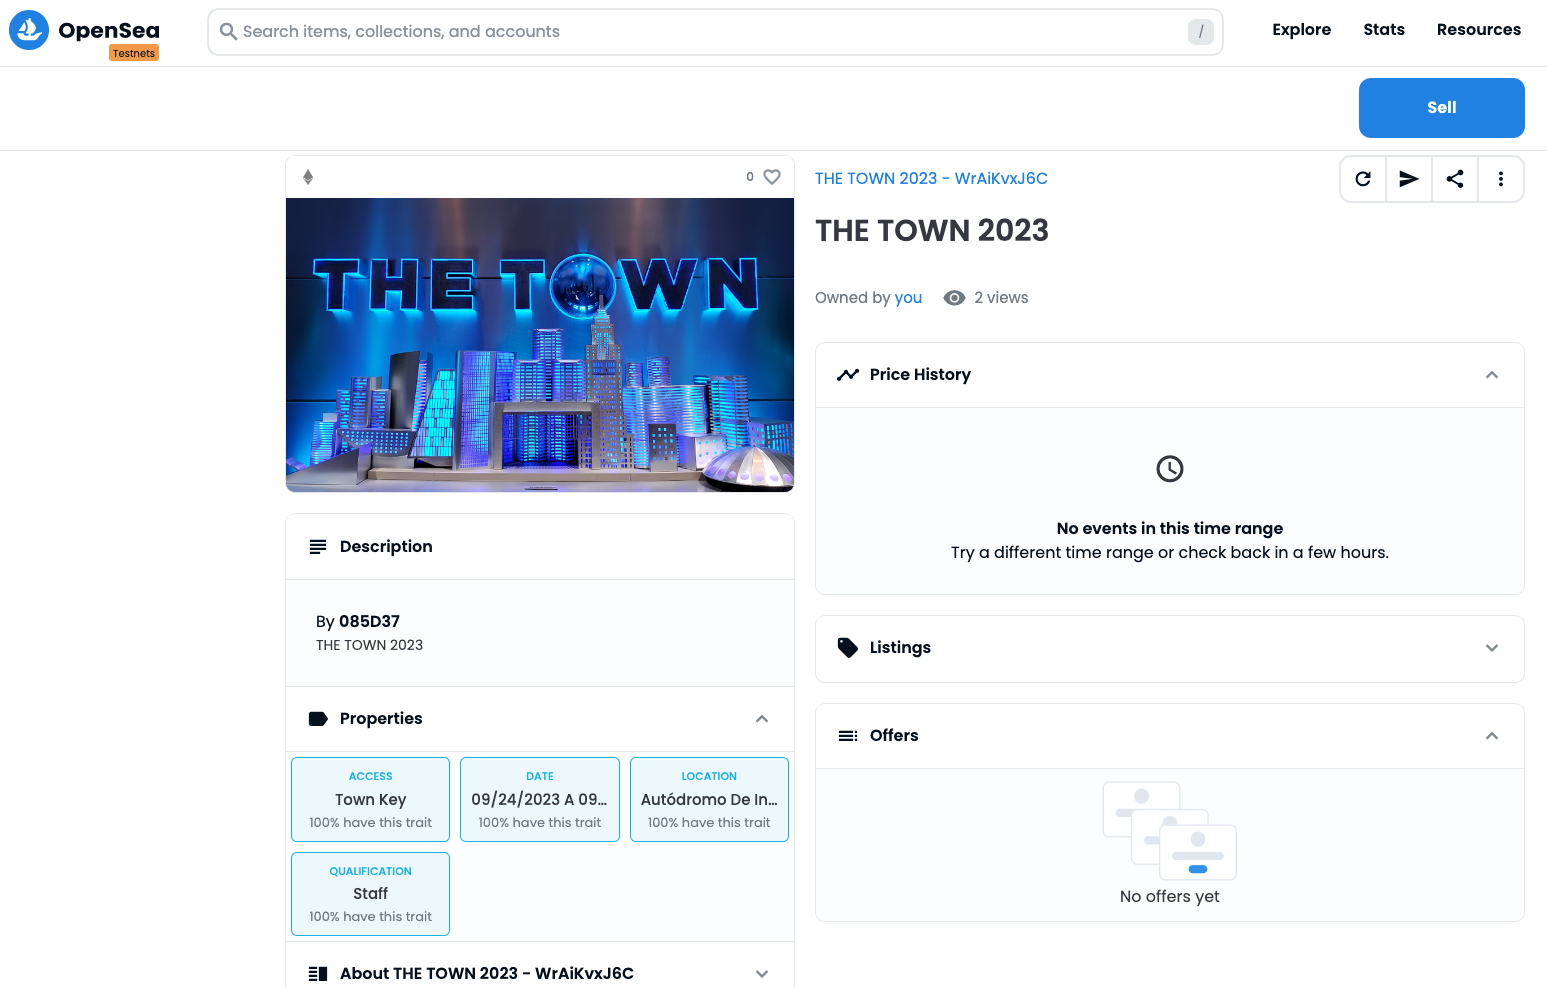
\includegraphics[scale=0.25]{figuras/opensea.png}
    \label{fig:opensea}
\end{figure}

\subsection{\esp Livre tráfego do ativo na rede}

Para demonstrar a posse efetiva do ativo por parte do consumidor, será feita uma transferência à um endereço de carteira terceira \footnote{Endereço: 0xc3d5C17877EfBD914a34281a8F6AD0874f826Bbe}, de modo que saia completamente do escopo de endereços conhecidos pelo domínio da aplicação sendo feita, inclusive, por meio da própria interface do \textit{OpenSea}, conforme demonstrado pela Figura \ref{fig:opensea-transfer}. A operação precisará ser aprovada utilizando a \textit{Metamask} antes de ser efetivada, já que o \textit{OpenSea} não tem acesso à chave privada da carteira, obrigando a intervenção, por segurança, porém não aumentando a complexidade para o usuário já que acontece de maneira fluida nas telas da plataforma.

\begin{figure}[ht]
    \centering
    \caption{\textit{OpenSea} - Transferência de ativo}
    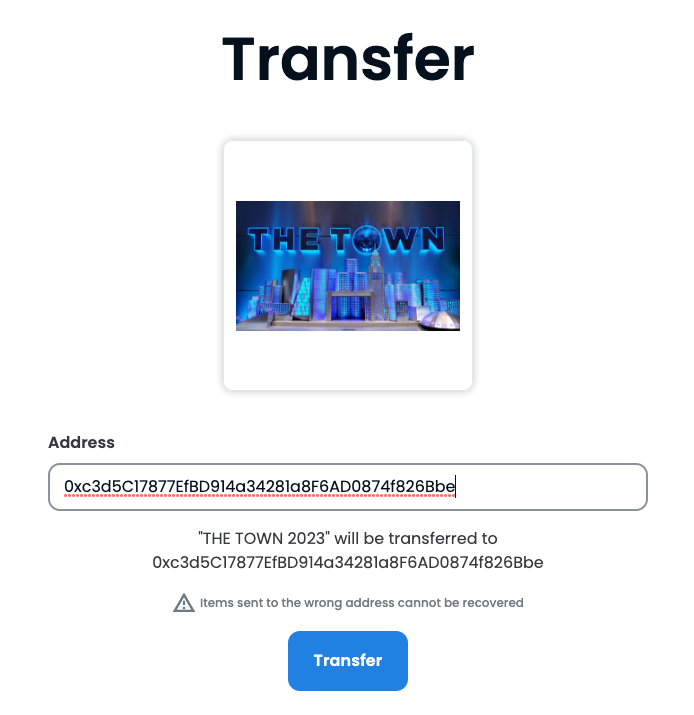
\includegraphics[scale=0.25]{figuras/opensea-transfer.png}
    \label{fig:opensea-transfer}
\end{figure}
    
\subsection{\esp Utilização de ingresso que foi transferido}

Para que um \textit{token} seja utilizado como ingresso, é necessário que ele esteja armazenado em um dos endereços da \textit{wallet} interna da aplicação. Sendo assim, após ser transferido para carteira proprietária -- e de lá para qualquer outro endereço --, eventualmente é necessário que este \textit{token} retorne para um dos endereços internos. 

Uma alternativa, não abordada por este artigo, seria fazer a verificação da posse do ativo por meio de uma transação, onde o usuário provaria a propriedade por meio de sua chave privada assinando uma transação aprovada pela rede, evitando que o consumidor precise transferir o \textit{NFT} de volta à um dos endereços internos da aplicação. Esta abordagem, porém, não foi adotada por exigir que o usuário tenha acesso à internet no momento da entrada, além de ser uma operação que dispoe de tempo -- algo que nem sempre está disponível no momento de acesso à um evento -- já que exige consenso da rede \textit{Ethereum}.

O consumidor que for o dono atual de um \textit{token} deve registrar (caso não tenha) uma conta na aplicação, habilitando que solicite qual o seu endereço interno. Com isso, ele deverá apenas fazer a transferência do seu \textit{NFT} -- vinda de qualquer carteira -- para o endereço informado pela plataforma, que identificará automaticamente a transação e atribuirá o ingresso correspondente àquele token para aquele consumidor. A partir daí, o consumidor utiliza o ingresso seguindo os mesmos passos descritos na \ref{ticket-utilization}.

A identificação automática da transação se dá por uma técnica de \textit{log processing}, de maneira que sejam rastreados constantemente os eventos de cada \textit{smart contract} implantado pelo sistema. Quando há uma transferência vinda de fora para quaisquer dos endereços internos, é feita a busca do consumidor associado ao endereço e o vínculo do \textit{token} com a conta se concretiza. Uma transferência só é dada como confirmada -- sendo considerada para o vínculo -- após a confirmação de 2 blocos, de maneira que a probabilidade de que a transação seja desfeita pela rede seja diminuída porém mantendo um tempo razoável de resposta em um ambiente de testes. Eventualmente, num ambiente produtivo, é recomendável que se aguarde, no mínimo, 12 blocos de confirmação.

\section{\esp Conclusão}

A proposta desse artigo foi investigar um problema de mercado -- corroborado pela pesquisa de campo realizada (apêndice \ref{pesquisa}) --  e defender uma solução com uso da tecnologia \textit{blockchain}. Apesar de ser um tema relevante e em constante ascensão, a colaboração dos \textit{NFTs} para o mercado de bilheteria online não possui muitas referências acadêmicas, apesar de ser um assunto que instiga e anima entusiastas dessa novidade, sendo extremamente necessário que uma dose de conhecimento científico se responsabilize por tornar organizações que desejem implementar essa ideia mais conscientes das lacunas que ainda precisam ser preenchidas.

Uma delas é o sistema de pagamento inserido no aplicativo e suas limitações. Além de permitir transações por transferência direta ou cartão de crédito, uma sugestão válida é inserir as criptomoedas como forma de pagamento de ingressos no futuro, como \textit{Bitcoin} ou \textit{Ether}. Essa ideia precisa levar em conta a dinâmica desses mercados paralelos, já que um ticket adquirido através das criptomoedas pode ter valores diferentes e a paridade de valores precisa ter motivações o bastante para ser justa e coerente.

Além disso, existe a possibilidade de os ingressos utilizados serem transformados em \textit{NFTs} como suvenir, uma lembrança da experiência, sem a possibilidade de serem usados novamente. Isso exige que o \textit{QR Code} e todas os mecanismos de validação sejam devidamente desativados, impedindo que outra pessoa utilize esse mesmo ingresso.

Os tipos de \textit{tickets} possíveis para essa novidade são variados e se houver incentivos para que mais categorias sejam formuladas pelo criador do evento isso deve ser realizado. Pode-se, inclusive, sugerir diferentes comissões para cada tipo de ingresso, incentivando a oferta qualificada. Ademais, não é só esperado, mas sugerido que um melhor desenvolvimento do \textit{FrontEnd} ocorra com foco na experiência do usuário e jornada de compra, facilitando e incentivando o uso de todas as ferramentas disponíveis na aplicação.
    
A apresentação dessa dor de mercado não busca apenas justificar a existência dessa aplicação, mas fundamentar futuras investigações a respeito do comércio secundário de bilheterias online, contribuindo para outras soluções nas mais diversas áreas do conhecimento. As informações expostas também pretendem incentivar a absorção da tecnologia \textit{blockchain}, assim como o uso de \textit{NFTs}, nos mais diversos âmbitos, já que, como se comprovou, é um artifício seguro e dotado de muitas possibilidades.